\providecommand{\main}{../..}
\documentclass[\main/dresen_thesis.tex]{subfiles}

\begin{document}
\chapter{Loosely-packed nanostructures}\label{ch:looselyPackedNS}
Magnetic nanospheres are nowadays routinely synthesized from a large choice of materials \cite{Gubin_2005_Magne}.
Magnetite ($\ch{Fe3O4}$) is a common choice for the study of nanomagnetism as it shows strong ferromagnetism and is widely available.
Due to extensive research, it is now possible to synthesize iron oxide nanoparticles that are highly tunable in size and shape \cite{Wetterskog_2014_Preci}.
In this work, two batches of iron oxide nanospheres in the size range of $11 \unit{nm}$ (IOS-11) and $7 \unit{nm}$ (IOS-7) are studied for their individual structural and magnetic properties.
Furthermore, loosely packed layers of the nanoparticles, created by spin coating the particles from dispersion on a substrate, are studied.
The magnetic properties of the nanostructure are compared to the individual nanoparticle properties and compared to model calculations to search for emergent effects arising from dipolar interparticle interaction.

\section{Spherical iron oxide nanoparticles}
Iron oxide nanoparticles were obtained from a collaboration with the group of Prof. Tremel from the inorganic chemistry department of the university of Mainz.
Briefly, they were prepared by following a popular synthesis route where first iron oleate is prepared from iron(III) chloride and then nanospheres are obtained by a controlled thermal decomposition of the oleate in a high boiling solvent (1-Octadecene).
A similar synthesis procedure is used in \refsec{ch:monolayers} for the preparation of cobalt ferrite nanocubes and is explained in that section in more detail.

\begin{figure}[tb]
  \centering
  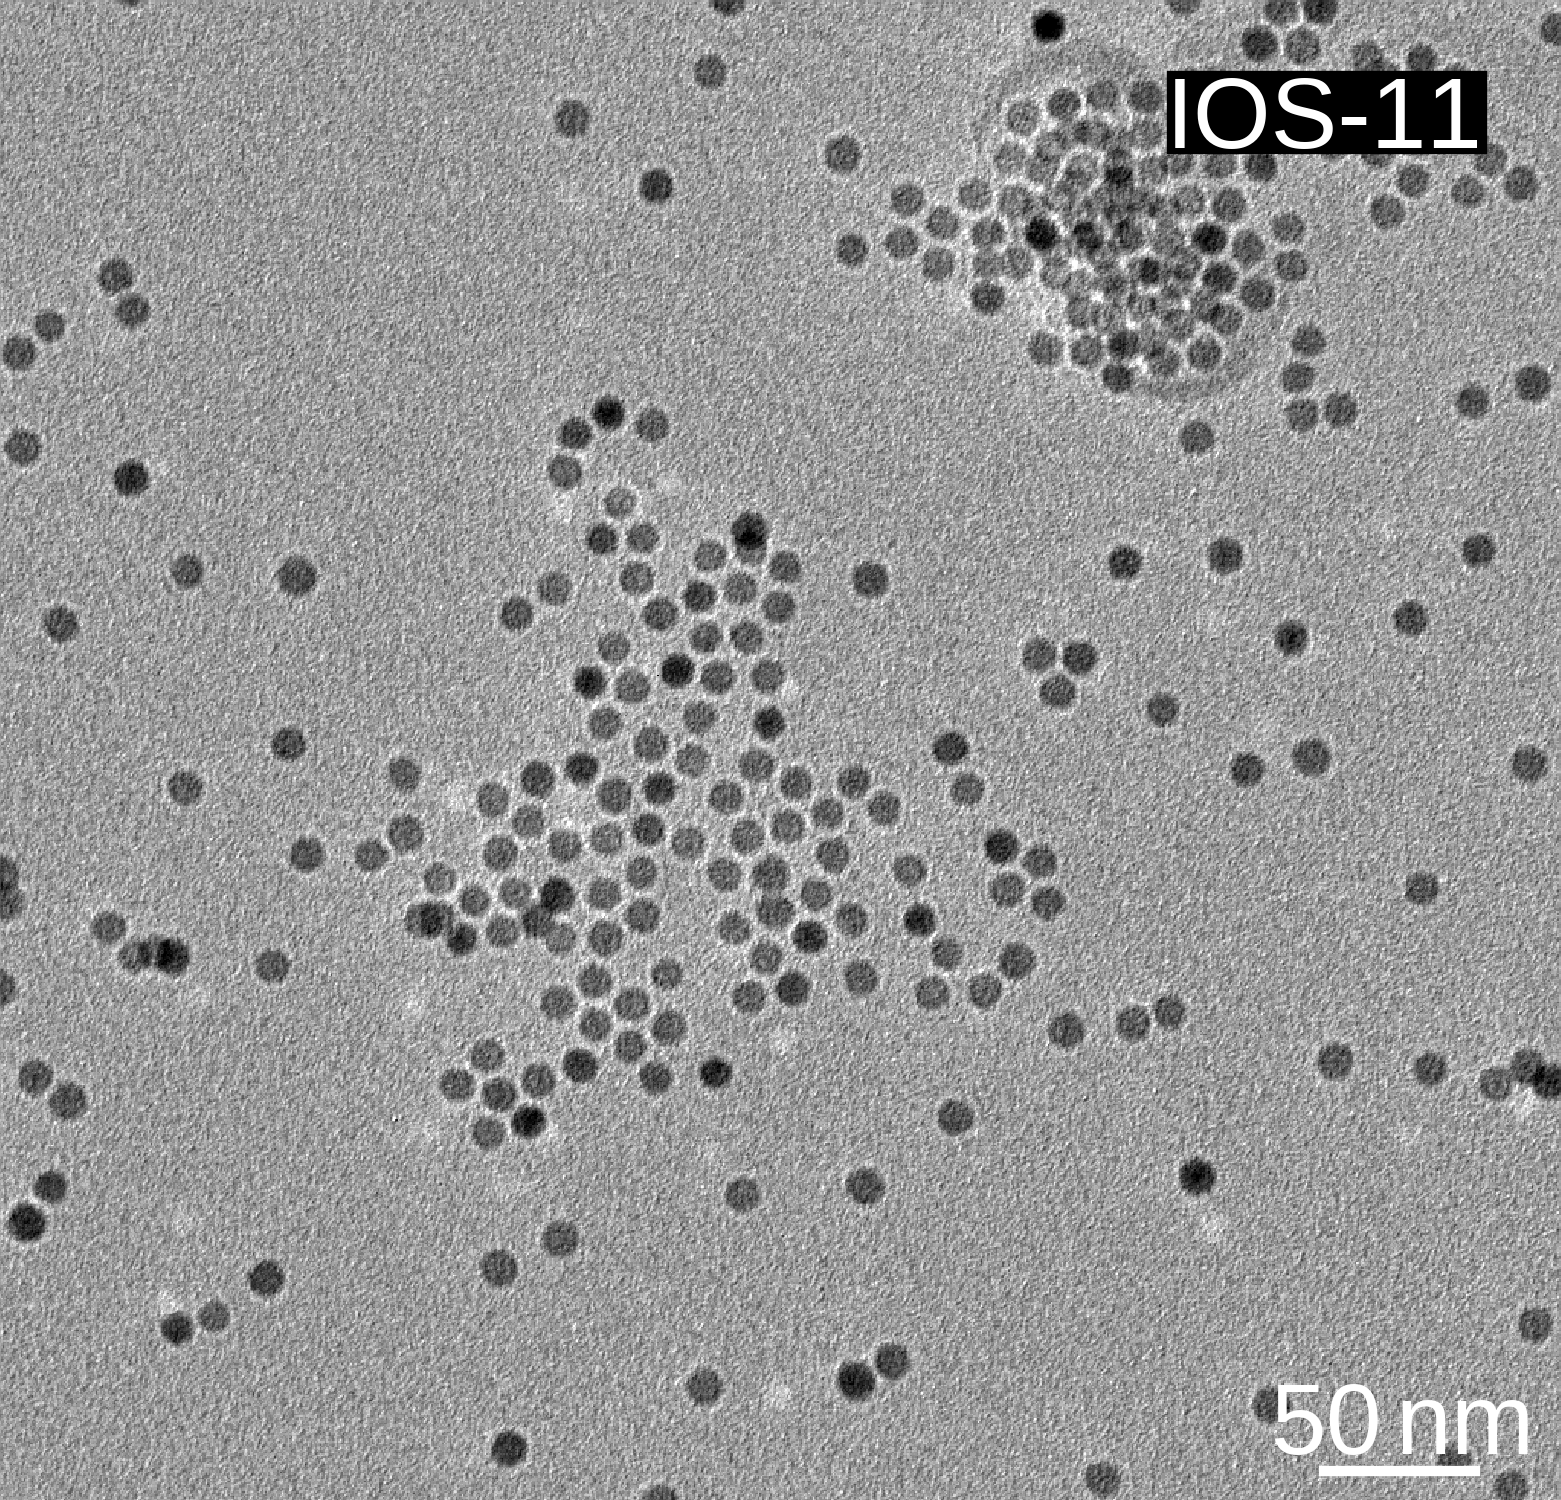
\includegraphics{looselyPackedNP_TEM_PMK18}
  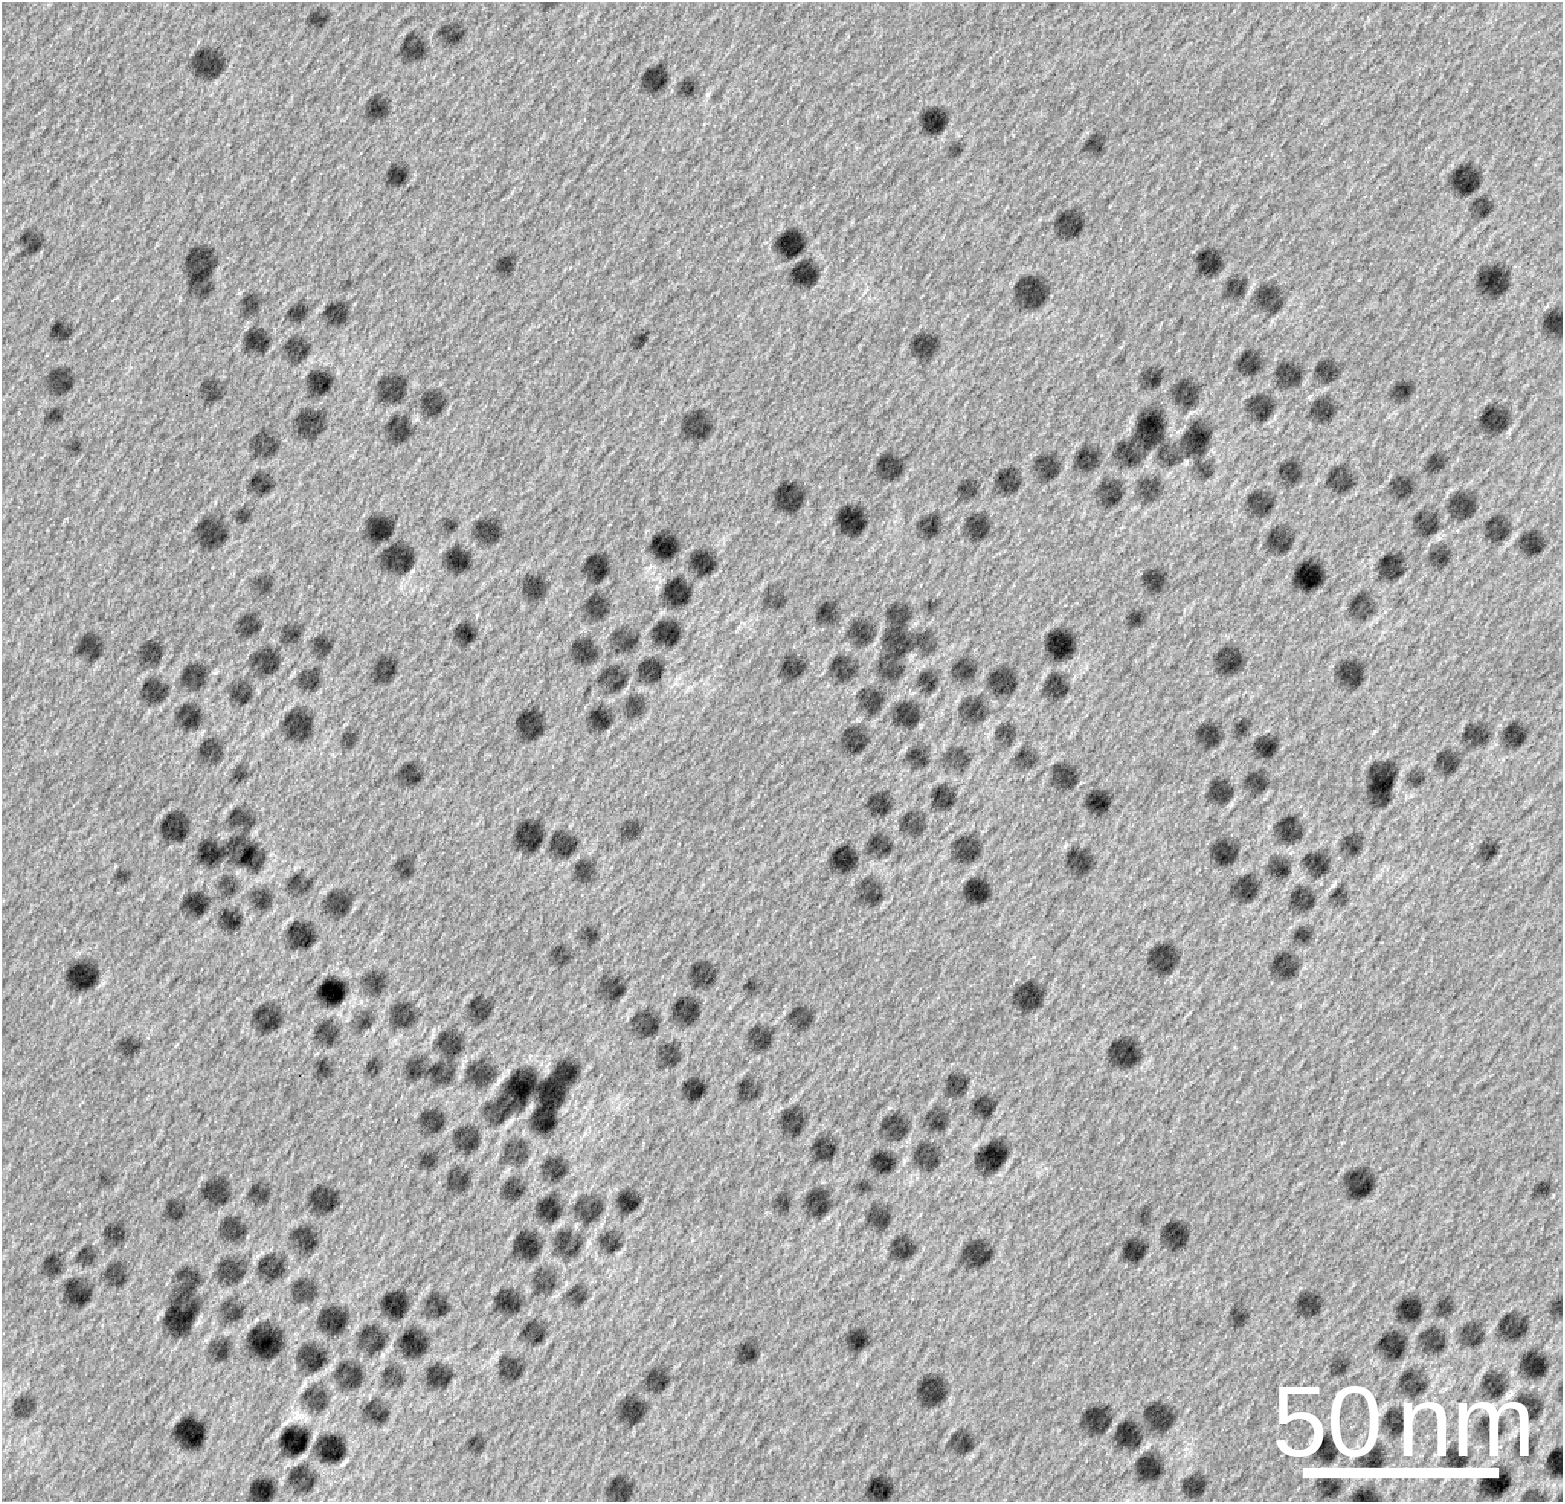
\includegraphics{looselyPackedNP_TEM_KWi338}
  \caption{\label{fig:looselyPackedNP:nanoparticle:tem}Transmission electron microscopy images of iron oxide nanospheres IOS-11 (left) and IOS-7 (right).}
\end{figure}

In a first step, the iron oxide nanospheres are characterized by transmission electron microscopy.
The measurements in \reffig{fig:looselyPackedNP:nanoparticle:tem} show the spherical shape of the nanoparticles.
By manually measuring the diameters of $\approx 200$ particles each, the probability density is estimated for both batches.
In \reffig{fig:looselyPackedNP:nanoparticle:temSizeDist}, the counted diameters are shown as histogram and both distributions are fit using the log-normal distribution
\begin{align}
  p(d; \mu, \sigma) \eq \frac{1}{\sqrt{2\pi} \sigma d} \exp \biggl( - \frac{\log(d) - \log(\mu)}{2 \sigma^2} \biggr),
\end{align}
where the parameters $\mu$ and $\sigma$ relate to the expectation value and standard deviation of the probability distribution via
\begin{align}
  E[d] \eq& \mu e^{\sigma^2/2} \approx \mu,\\
  Std[d] \eq& \mu e^{\sigma^2/2} \sqrt{e^{\sigma^2} - 1} \approx \mu \sigma,\\
\end{align}
with the approximations being valid for $\sigma^2 \ll 1$.
The log-normal distribution is generally used to model nanoparticle size distribution phenomenologically as it allows only for positive numbers.
With size distributions being commonly in the order of $10 \, \%$ in this work, it follows that the width parameter is $\sigma \approx \mathcal{O}(0.1)$ and therefore using the above approximations, $\mu$ can be treated as the expectation value and $\sigma$ as the relative standard deviation.

The batch IOS-11 is well described by a single log-normal function.
The second batch, however, has a broader size distribution and a bimodal log-normal distribution is better suited to describe the probability distribution
\begin{align}
  p_\mathrm{bimodal}(d) \eq \alpha p_1(d; \mu_1, \sigma_1) + (1 - \alpha) p_2(d; \mu_2, \sigma_2),
\end{align}
where $\alpha$ is the fraction of the first mode.
Here, the batch is described by being one part particles with a narrow size distribution and one part with a broad size distribution.
The estimated parameters for both samples are listed in \reftab{tab:looselyPackedNP:nanoparticle:temModel}.
\begin{figure}[tb]
    \centering
    \captionof{table}{\label{tab:looselyPackedNP:nanoparticle:temModel}Parameters estimated for the size distribution of IOS-11 and IOS-7 from fitting a (bimodal) log-normal size distribution.}
    \begin{minipage}{0.49\textwidth}
      \centering
      \begin{tabular}{ c | l | l }
          & IOS-11 & IOS-7 \\
        \hline
        $\alpha$    & $1$                   & $0.7(1)$   \\
        $\mu_1$     & $10.95(5) \unit{nm}$  & $6.97(6) \unit{nm}$ \\
        $\sigma_1$  & $6.6(4) \unit{\%}$    & $11(1) \unit{\%}$ \\
        $\mu_2$     & -                     & $6.0(6) \unit{nm}$ \\
        $\sigma_2$  & -                     & $29(4) \unit{\%}$ \\
        \hline
      \end{tabular}
    \end{minipage}
    \begin{minipage}{0.49\textwidth}
      \centering
      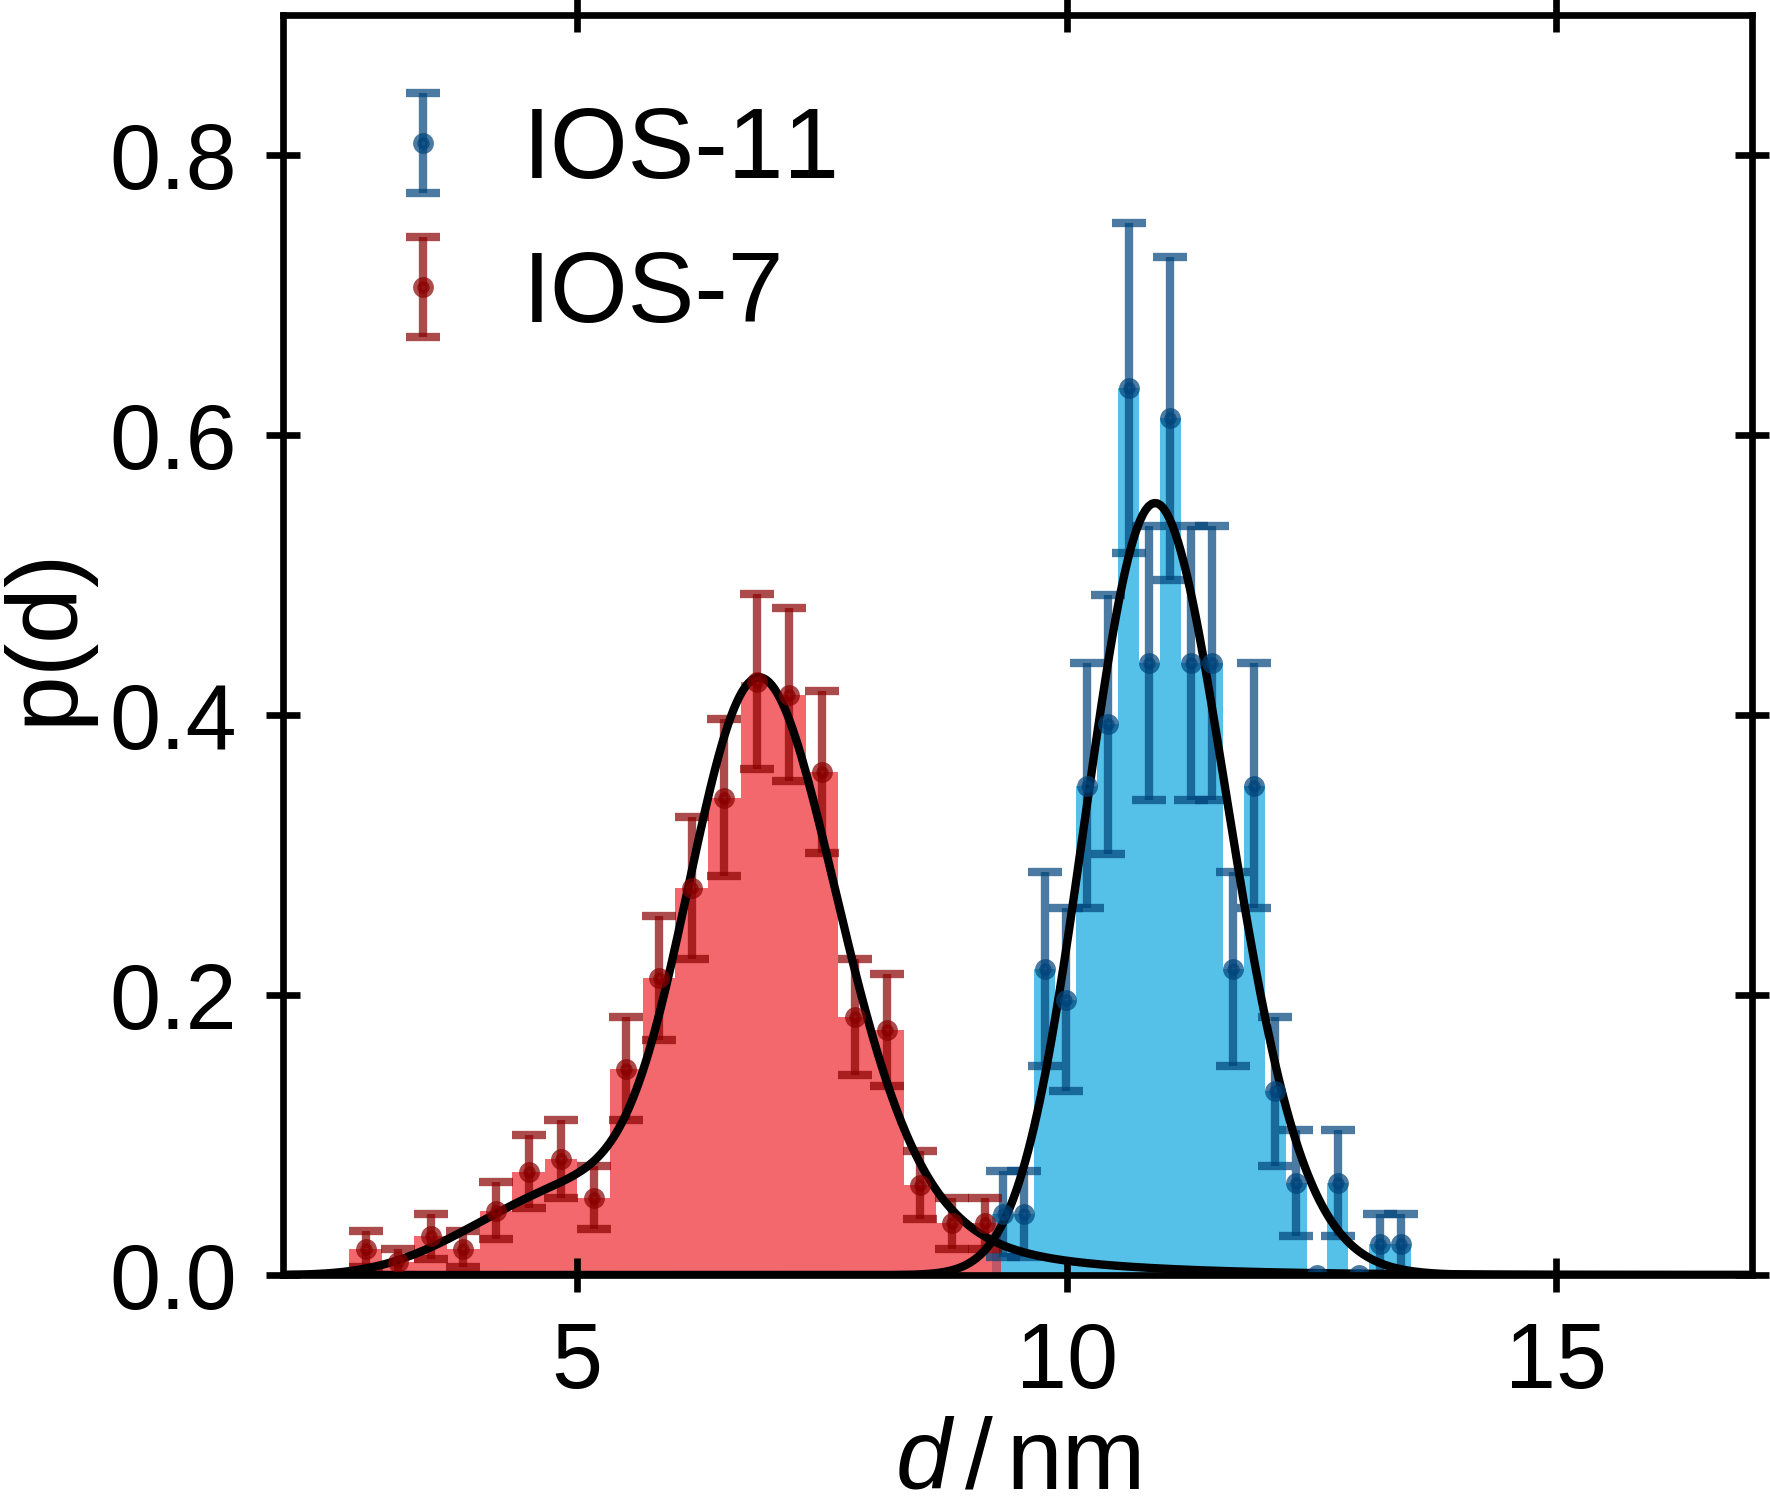
\includegraphics{looselyPackedNP_TEM_PMK18_KWi338_sizeDist}
    \end{minipage}
    \captionof{figure}{\label{fig:looselyPackedNP:nanoparticle:temSizeDist}Size distribution of IOS-7 and IOS-11 extracted from transmission electron microscopy by manually measuring the diameters.}
\end{figure}

Transmission electron microscopy allows to estimate the size from a local snapshot of the dry sample.
A better estimate to quantify the average particle size and size distribution in a dispersion is given by small-angle scattering.
As the particle beam, which has an extension of a few $100 \unitmu$, hits an volume of the dispersion that typically contains $\approx \mathcal{O} (10^{12})$ particles, the estimated parameters from modelling small-angle scattering data is much more representative for the average particle in dispersion than electron microscopy.

Small-angle x-ray scattering (SAXS) experiments were performed on both samples at the \textsc{GALAXI} instrument in the \textsc{Forschungszentrum J\"ulich}, which is described in \refapp{ch:appendix:lss:galaxi}.
Additionally, small-angle neutron scattering (SANS) experiments were performed on the same nanoparticles at the \textsc{D33} instrument at the \textsc{Institute Laue-Langevin} that is described in \refapp{ch:appendix:lss:d33}.
To determine the size of the particles, the data from both experiments is fitted simultaneously to one model.
The particles are modelled as spherical magnetite particles with a brush of oleic acid coated around them.
The particles were dispersed in cyclohexane for the SAXS experiment, and in deuterated toluene for the SANS experiment.
The solvents are chosen to increase the contrast with respect to the oleic acid in the case of SAXS and to minimize the incoherent scattering from hydrogen in the case of SANS.

As in the case of transmission electron microscopy, it is necessary for IOS-7 to add a second mode of particle sizes to the model.
Furthermore, to obtain a good model for the SANS data, it is necessary that the scattering length density of the oleic acid shell is allowed to vary freely between the bulk value for the solvent and the bulk value for oleic acid, as the solvent could mix in between the oleic acid brushes of the nanoparticles.
Free oleic acid in the solvent can form micelles, in the case of IOS-7 this has to be included in the model for a good fit of the data by adding another spherical form factor for particles with the radius and scattering length density equal to the shell of the nanoparticles.
The fit parameter $n_\mathrm{OA}$ quantifies then the number density of the oleic acid micelles in dispersion.
The best fit parameters are tabulated in \reftab{tab:looselyPackedNP:nanoparticle:sas} and the obtained sizes and size distributions by the model are in good agreement to the local result from electron microscopy.
Only the second mode of the IOS-7 batch is best fitted in the SAS data with a smaller diameter of $2.2 \unit{nm}$ and a size distribution of $56\,\%$ instead of the obtained $6 \unit{nm}$ and $29\,\%$ in electron microscopy.

\begin{figure}[tb]
  \centering
  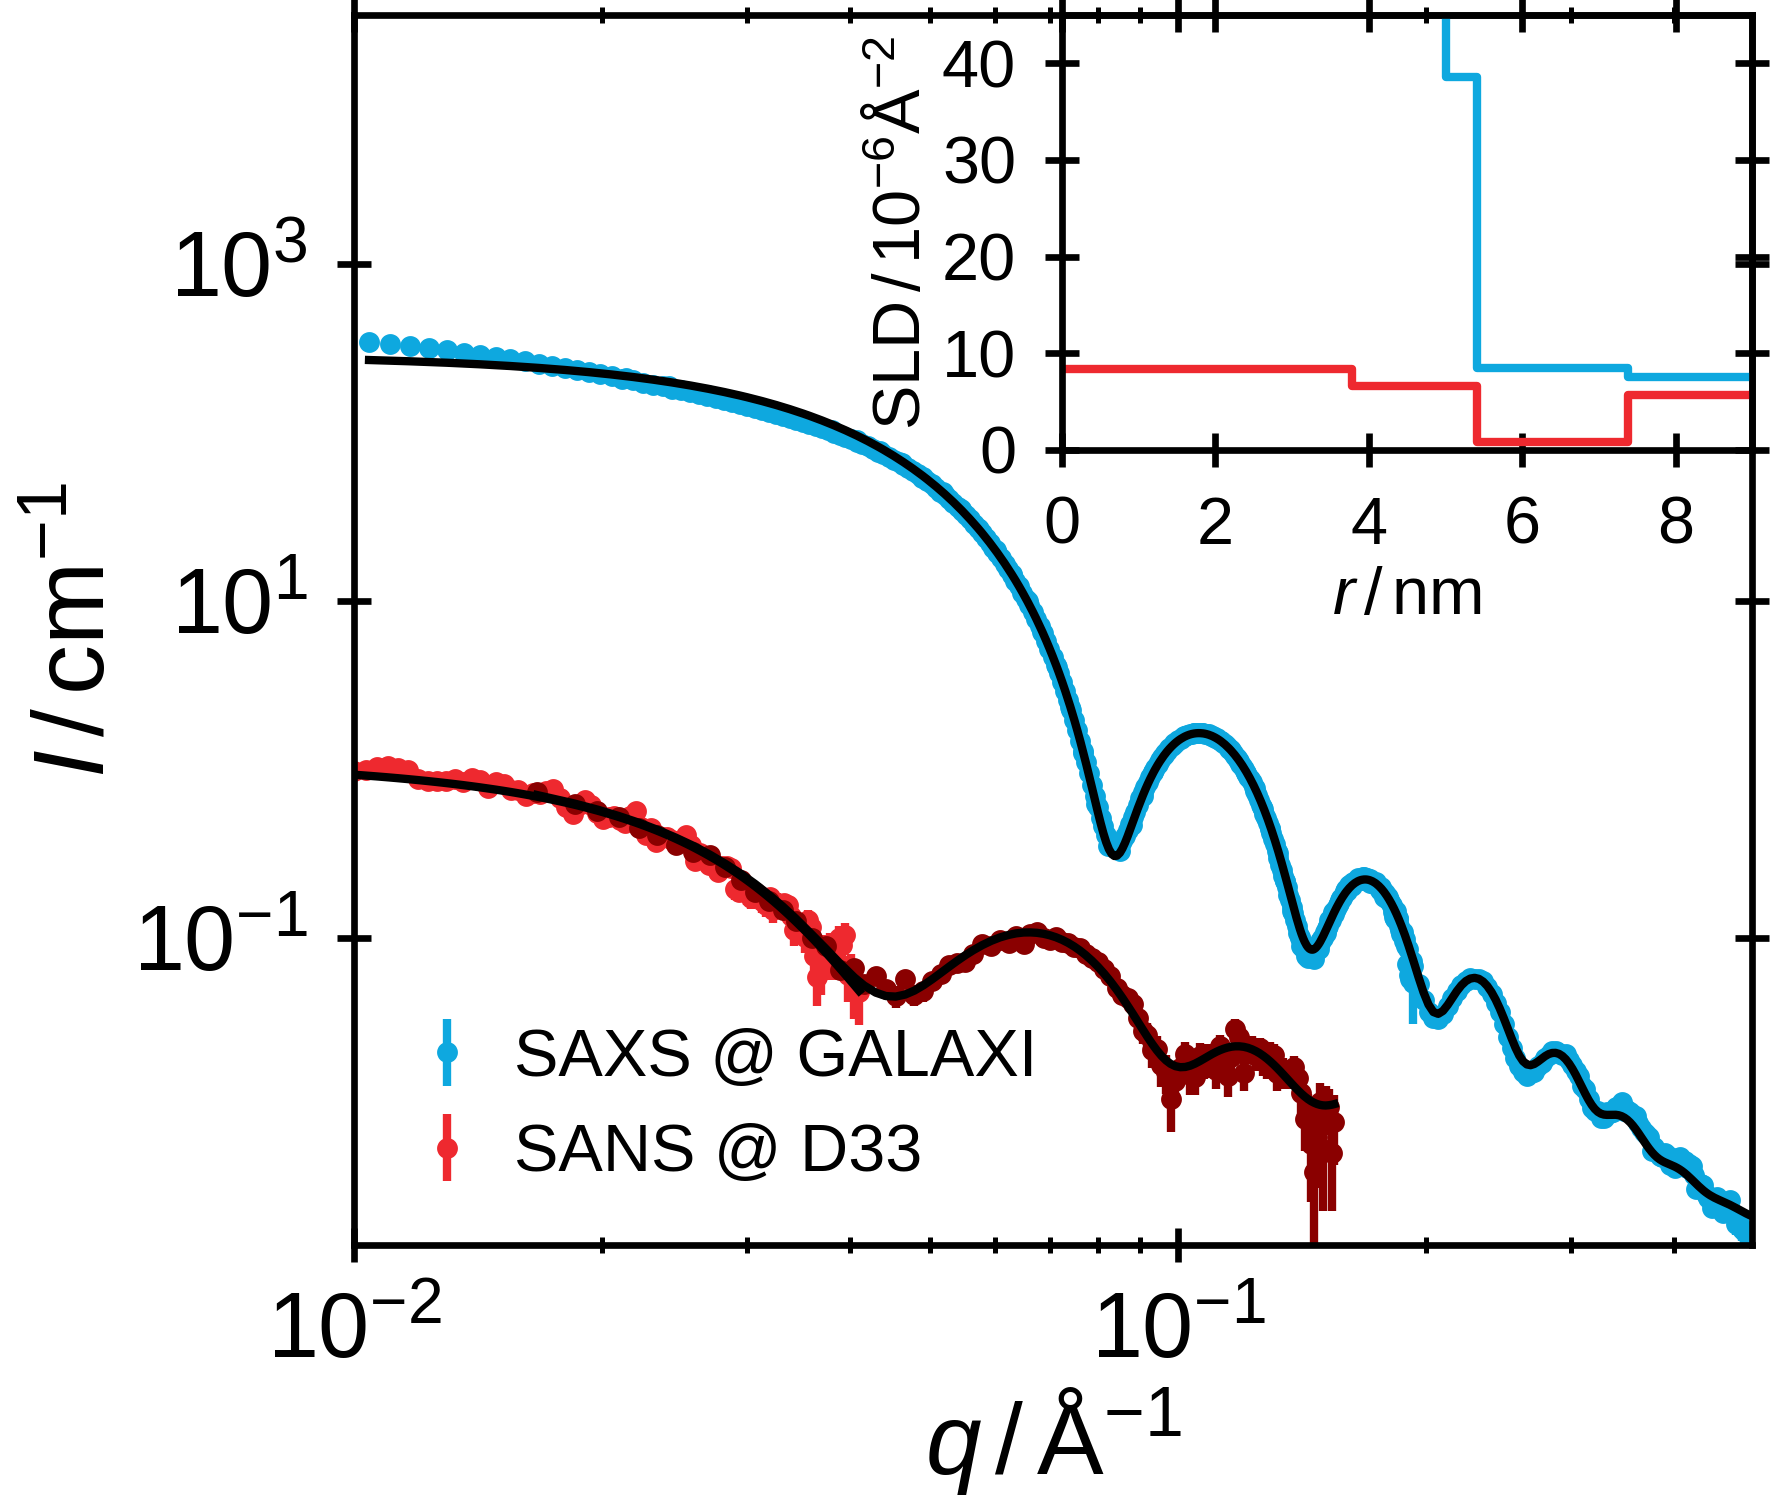
\includegraphics{looselyPackedNP_SAS_IOS-11_SASFit}
  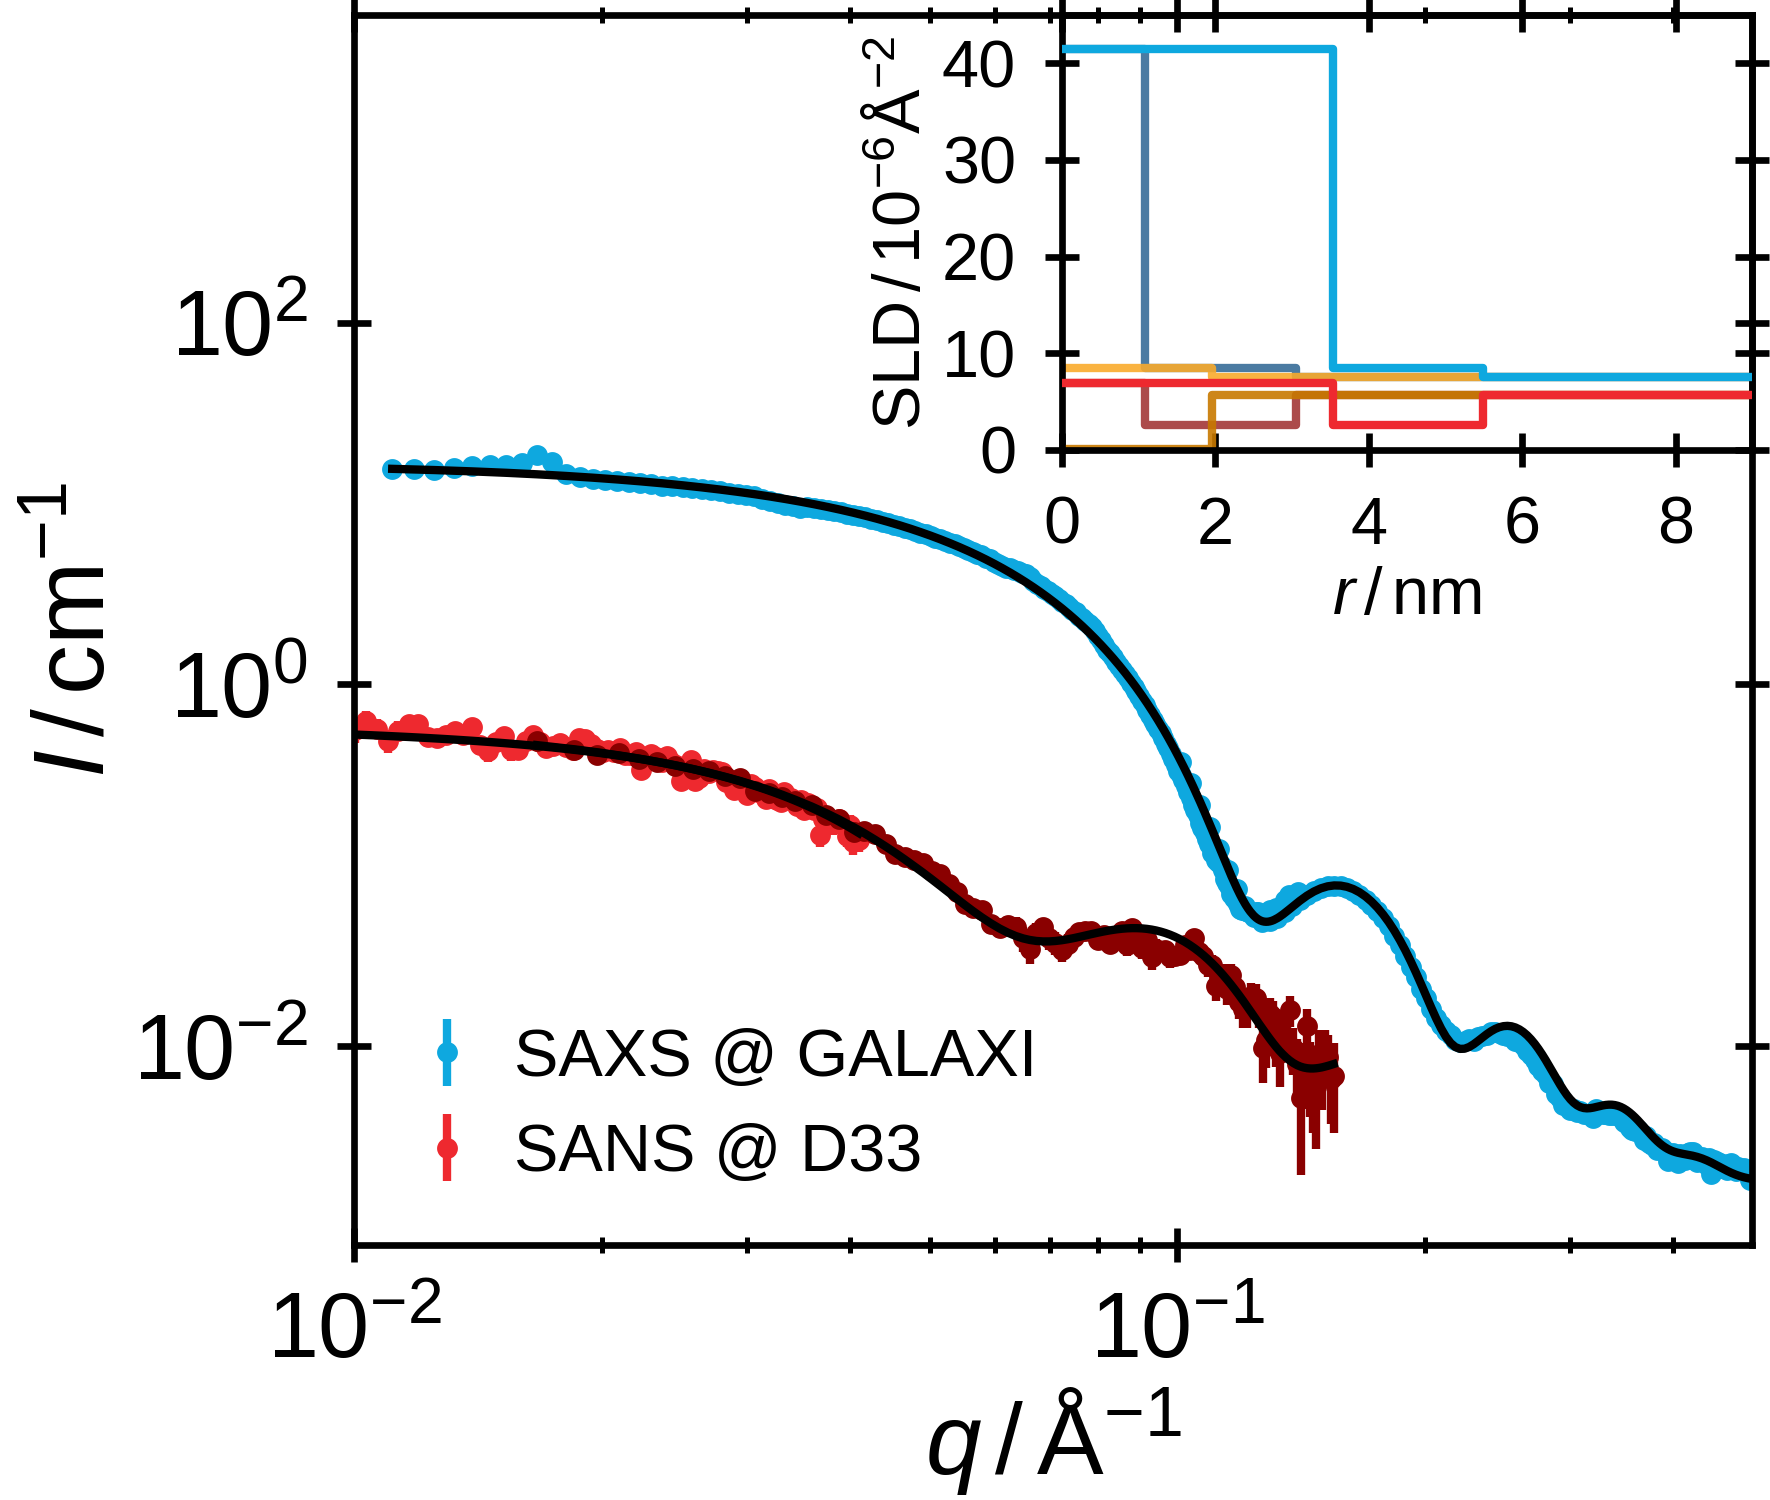
\includegraphics{looselyPackedNP_SAS_IOS-7_SASFit}
  \caption{\label{fig:looselyPackedNP:nanoparticle:sas}Small-angle x-ray and neutron scattering for IOS-11 (left) and IOS-7 (right). The x-ray and neutron datasets are fitted simultaneously to a spherical core-shell model to estimate the average size of the particle size and surfactant shell.}
\end{figure}

\begin{table}[tb]
  \centering
  \caption{\label{tab:looselyPackedNP:nanoparticle:sas}Parameters for the spherical core-shell model of IOS-11 and IOS-7.}
  \begin{tabular}{ c | l | l }
      & IOS-11 & IOS-7 \\
    \hline
    $R$
      & $5.276(8) \unit{nm}$
      & $3.53(1) \unit{nm}$\\
    $R_2$
      &
      & $1.00(2) \unit{nm}$\\
    $D$
      & $1.90(6) \unit{nm}$
      & $1.90 \unit{nm}$\\
    $\sigma_R$
      & $6.0(2) \,\%$
      & $6.8(9) \,\%$\\
    $\sigma_{R_2}$
      &
      & $59(4) \,\%$\\
    \hline
    $\alpha$
      & $1$\\
      & $40(4) \,\%$\\
    $n^\mathrm{saxs}$
      & $0.533(3) \cdot 10^{-8} \angstrom^{-3}$
      & $0.6(1) \cdot 10^{-8} \angstrom^{-3}$\\
    $bg^\mathrm{saxs}$
      & $0.009(1) \unit{cm}^{-1}$
      & $0.00134 \unit{cm}^{-1}$\\
    $n^\mathrm{sans}$
      & $0.27(1)\cdot 10^{-8} \angstrom^{-3}$
      & $0.73(9) \cdot 10^{-8} \angstrom^{-3}$\\
    $\rho_\mathrm{shell}^\mathrm{sans}$
      & $2.6(1) \cdot 10^{-6} \angstrom^{-2}$
      & $2.6    \cdot 10^{-6} \angstrom^{-2}$\\
    $\Delta \theta_\mathrm{s. a.}$
      & $0.0031(2)$
      & $0.0031$\\
    $\Delta \theta_\mathrm{l. a.}$
      & $0.0036(2)$
      & $0.0036$\\
    $n_\mathrm{OA}$
      &
      & $0.66(8) \cdot 10^{-8} \angstrom^{-3}$\\
    \hline
    $\rho_\mathrm{core}^\mathrm{saxs}$
      & \multicolumn{2}{c}{$41.469 \cdot 10^{-6} \angstrom^{-2}$}\\
    $\rho_\mathrm{shell}^\mathrm{saxs}$
      & \multicolumn{2}{c}{$8.514 \cdot 10^{-6} \angstrom^{-2}$}\\
    $\rho_\mathrm{solvent}^\mathrm{saxs}$
      & \multicolumn{2}{c}{$7.554 \cdot 10^{-6} \angstrom^{-2}$}\\
    $\rho_\mathrm{core}^\mathrm{sans}$
      & \multicolumn{2}{c}{$6.941 \cdot 10^{-6} \angstrom^{-2}$}\\
    $\rho_\mathrm{solvent}^\mathrm{sans}$
      & \multicolumn{2}{c}{$5.664 \cdot 10^{-6} \angstrom^{-2}$}\\
    $bg^\mathrm{sans}$
      & \multicolumn{2}{c}{$0 \unit{cm}^{-1}$}\\
      $\lambda^\mathrm{sans}$
        & \multicolumn{2}{c}{$5.9984 \unit{\angstrom}$}\\
      $\Delta \lambda / \lambda ^\mathrm{sans}$
        & \multicolumn{2}{c}{$4.247 \, \%$}\\
    \hline
  \end{tabular}
\end{table}

To study the magnetic structure of the nanoparticles, vibrating sample magnetometry (VSM) is applied to measure the macroscopic magnetization of a dispersion as described in \refapp{app:additionalExperimentalTechniques:vsm} and polarized small-angle neutron scattering (SANSPOL) is applied to measure the magnetic scattering of the individual nanoparticles.
Both techniques allow to model the average individual nanoparticle magnetization and the results should be in agreement with one another.

For SANSPOL, a magnetic field of $B\eq 515 \unit{mT}$ was applied perpendicular \& horizontal to the beam direction and the scattered neutrons are counted on a position-sensitive detector for up and down polarized neutrons without polarization analysis after the scattering.
The same model and parameters as obtained from the nuclear small-angle scattering is used and extended by a spherical magnetic form factor.
The magnetic SLD of the core is fitted as parameter and possibly it is allowed that the magnetic radius of the particle is smaller by a size of $d_\mathrm{dead}$ due to a magnetically dead surface layer.
From the magnetic SLD, the volume magnetization is calculated using \refeq{eq:theoreticalBackground:scattering:magneticSLD}
\begin{align}
  M \eq& \mu_B s_e \eq \frac{2 \pi \hbar^2}{m_n \mu_0 \mu_n} \rho_\mathrm{mag},\\
  \frac{M}{[\unit{kA m^{-1}}]} \eq& 343.592 \cdot \frac{\rho_\mathrm{mag}}{[10^{-6} \angstrom^{-2}]}.
\end{align}
The obtained model is shown in \reffig{fig:looselyPackedNP:nanoparticle:sanspol} and the results in \reftab{tab:looselyPackedNP:nanoparticle:vsmSanspol}.

\begin{figure}[tb]
  \centering
  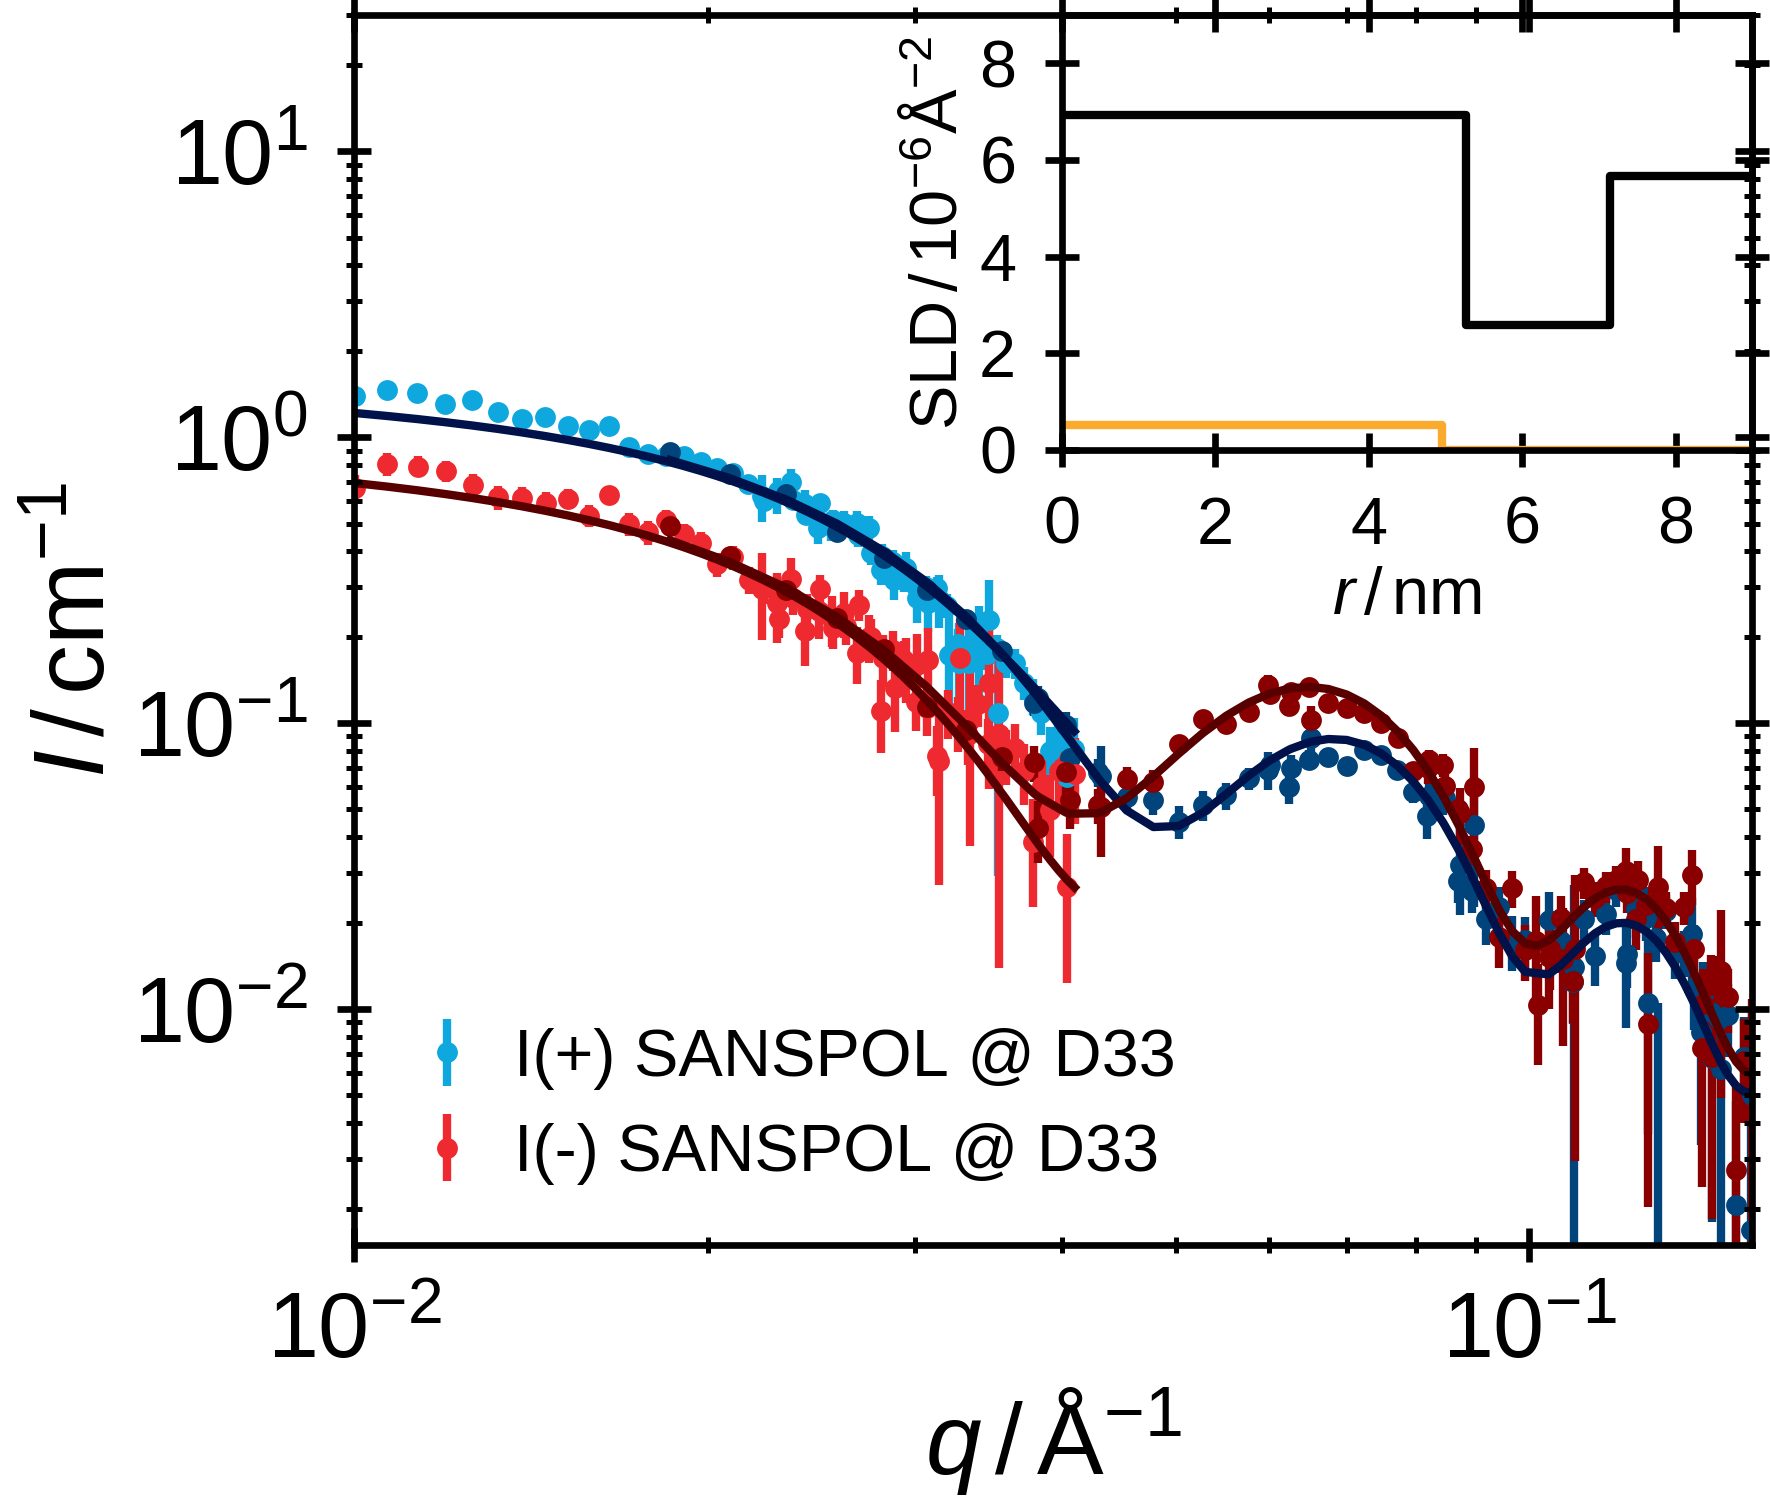
\includegraphics{looselyPackedNP_SAS_IOS-11_SANSPOLFit}
  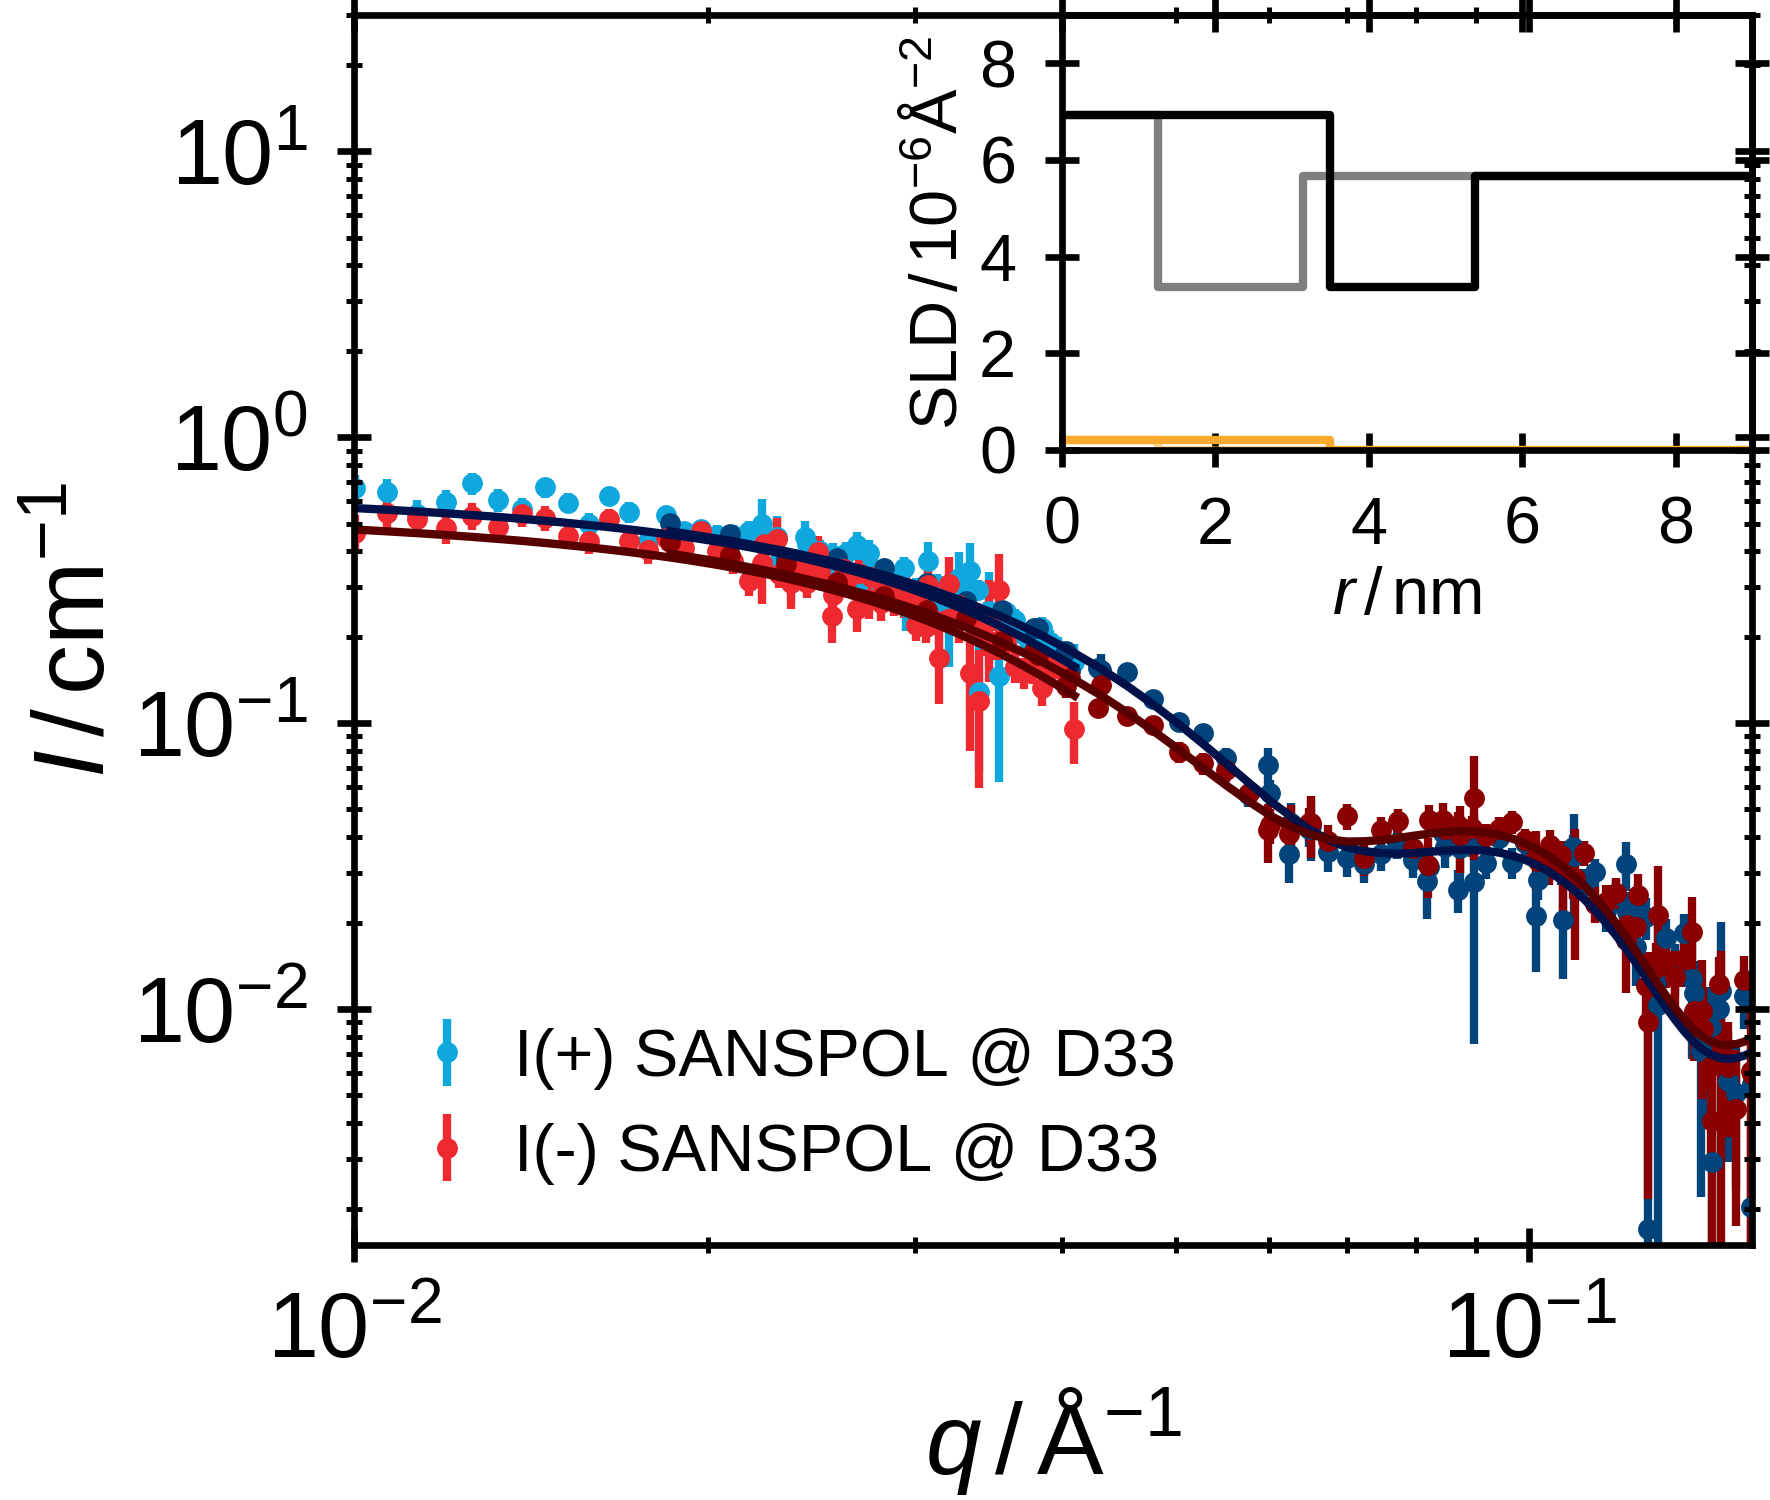
\includegraphics{looselyPackedNP_SAS_IOS-7_SANSPOLFit}
  \caption{\label{fig:looselyPackedNP:nanoparticle:sanspol}Polarized small-angle neutron scattering for IOS-11 (left) and IOS-7 (right).}
\end{figure}


For the VSM data, it is assumed that the dispersion is compromised of homogeneously magnetized, non-interacting particles that can be represented by a single classical super spin.
In \refapp{ch:appendix:calculations:magnetizationClassicalSpin}, it is shown that in this case the magnetization is given by a Langevin curve
\begin{align}
  M(H) \eq& M_s \biggl( \coth \biggl(\frac{\mu \mu_0 H}{k_B T} \biggr) - \frac{k_B T}{\mu \mu_0 H} \biggr) + \chi H.
\end{align}
Here, $M_s$ is the saturation magnetization, $\mu$ the magnetic moment of one nanoparticle and $\chi$ the excess susceptibility.
To properly obtain the saturation magnetization in units of $\unit{kAm{-1}}$, the exact volume of magnetic material in dispersion needs to be known and the measured magnetization data scaled accordingly.
The volume of the magnetic material can be estimated either by gravimetric methods or also by using the results obtained from small-angle scattering.
As one parameter in the small-angle scattering model is the number of particles per volume $n \eq N/V$ and another the volume of the particle $V_p$, the magnetic volume per dispersion volume is given by
\begin{align}
  \alpha \eq \frac{N V_p}{V}.
\end{align}
This ratio is multiplied with the volume of dispersion measured in the VSM experiment to obtain the volume that the final data is scaled to.
The data and best-fit model are shown in \reffig{fig:looselyPackedNP:nanoparticle:vsm} and the numerical values are given in \reftab{tab:looselyPackedNP:nanoparticle:vsmSanspol}.

\begin{figure}[tb]
  \centering
  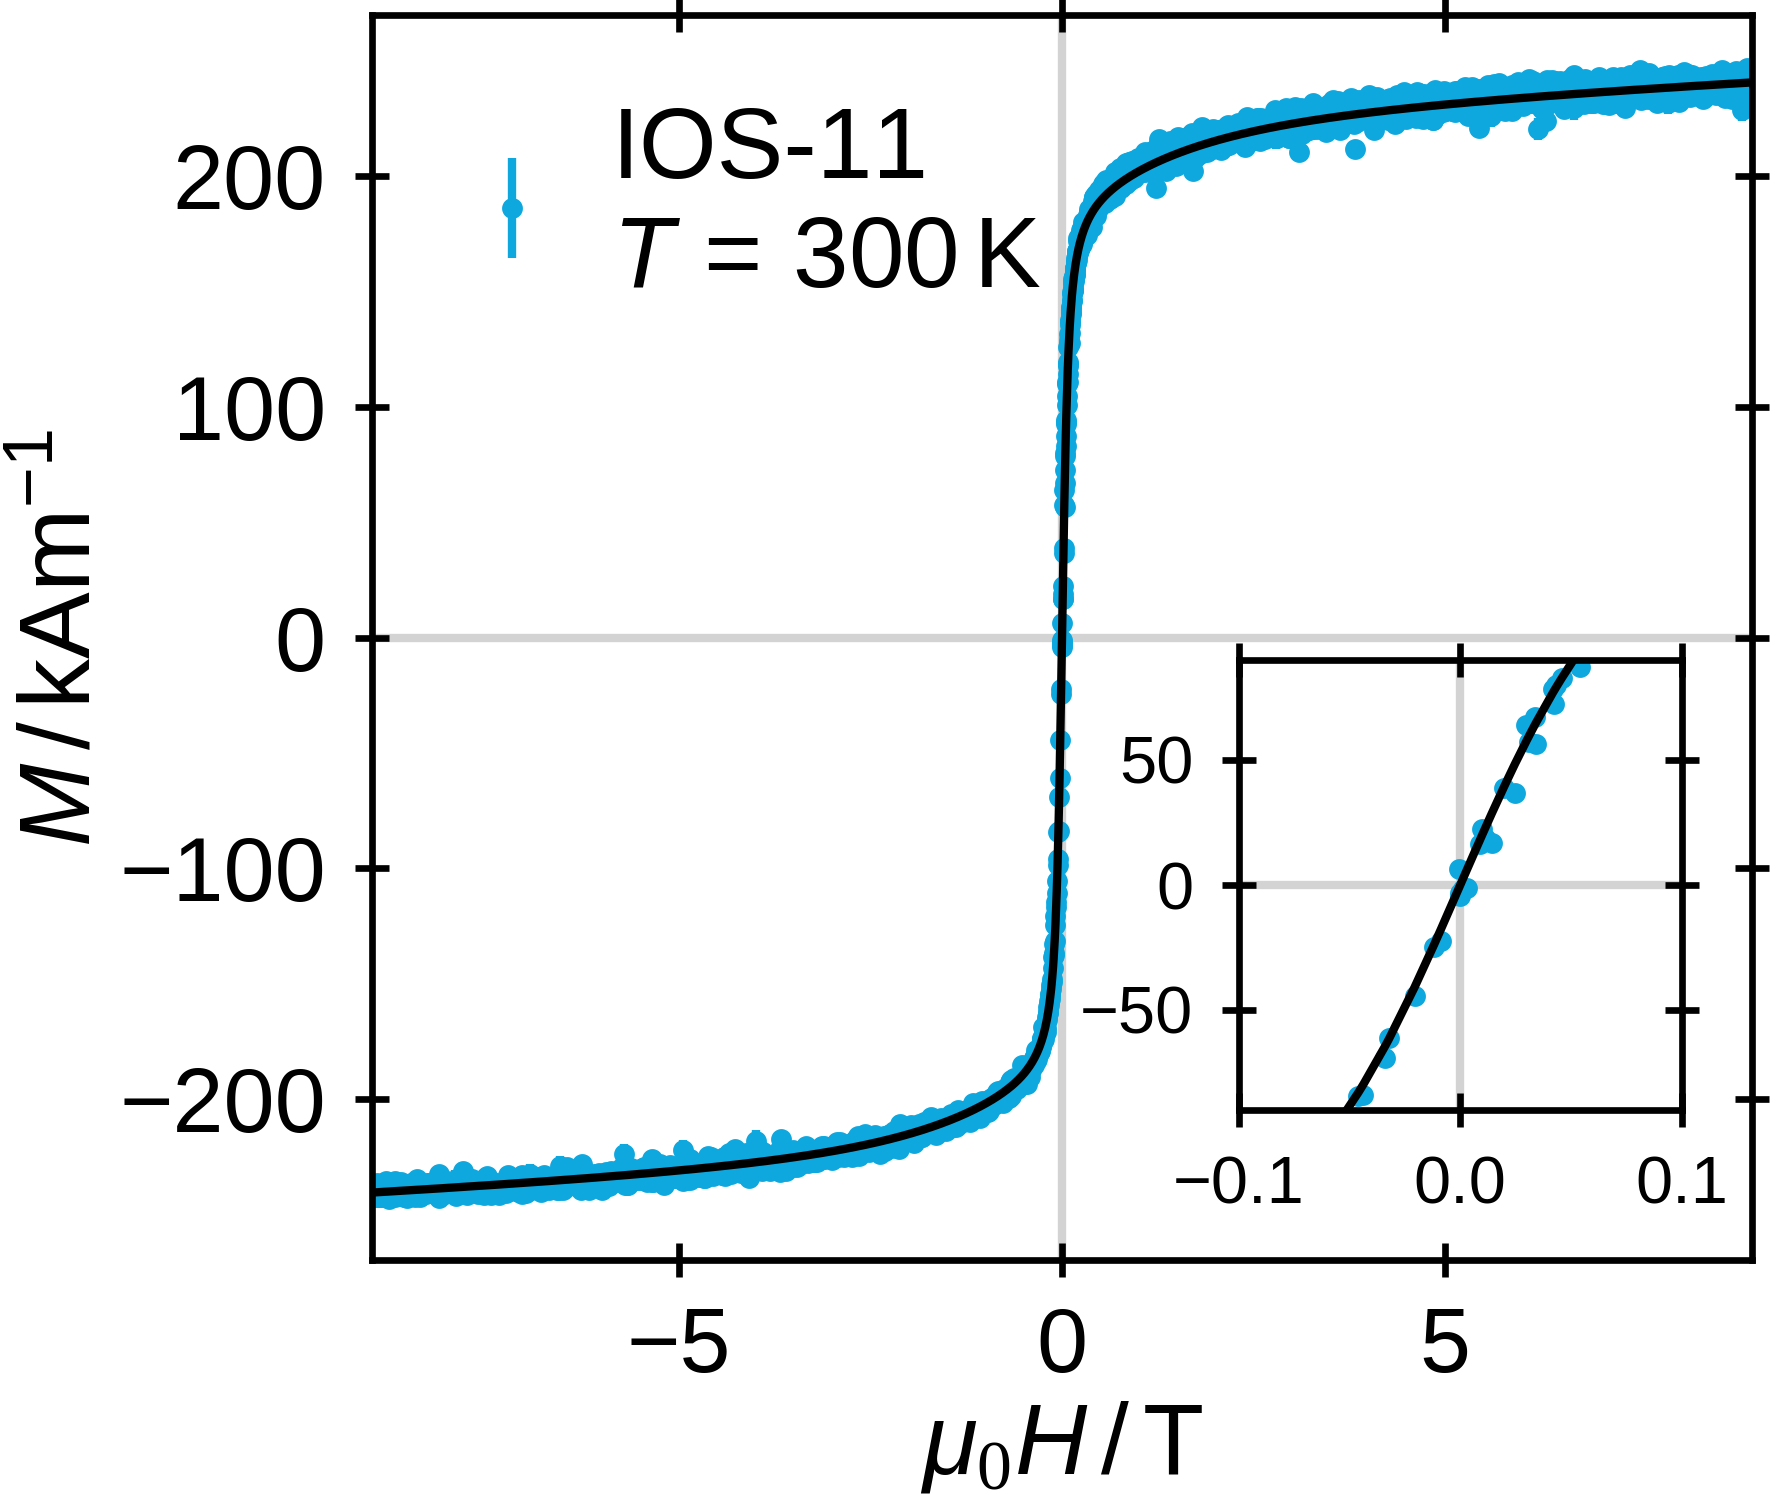
\includegraphics{looselyPackedNP_VSM_IOS-11}
  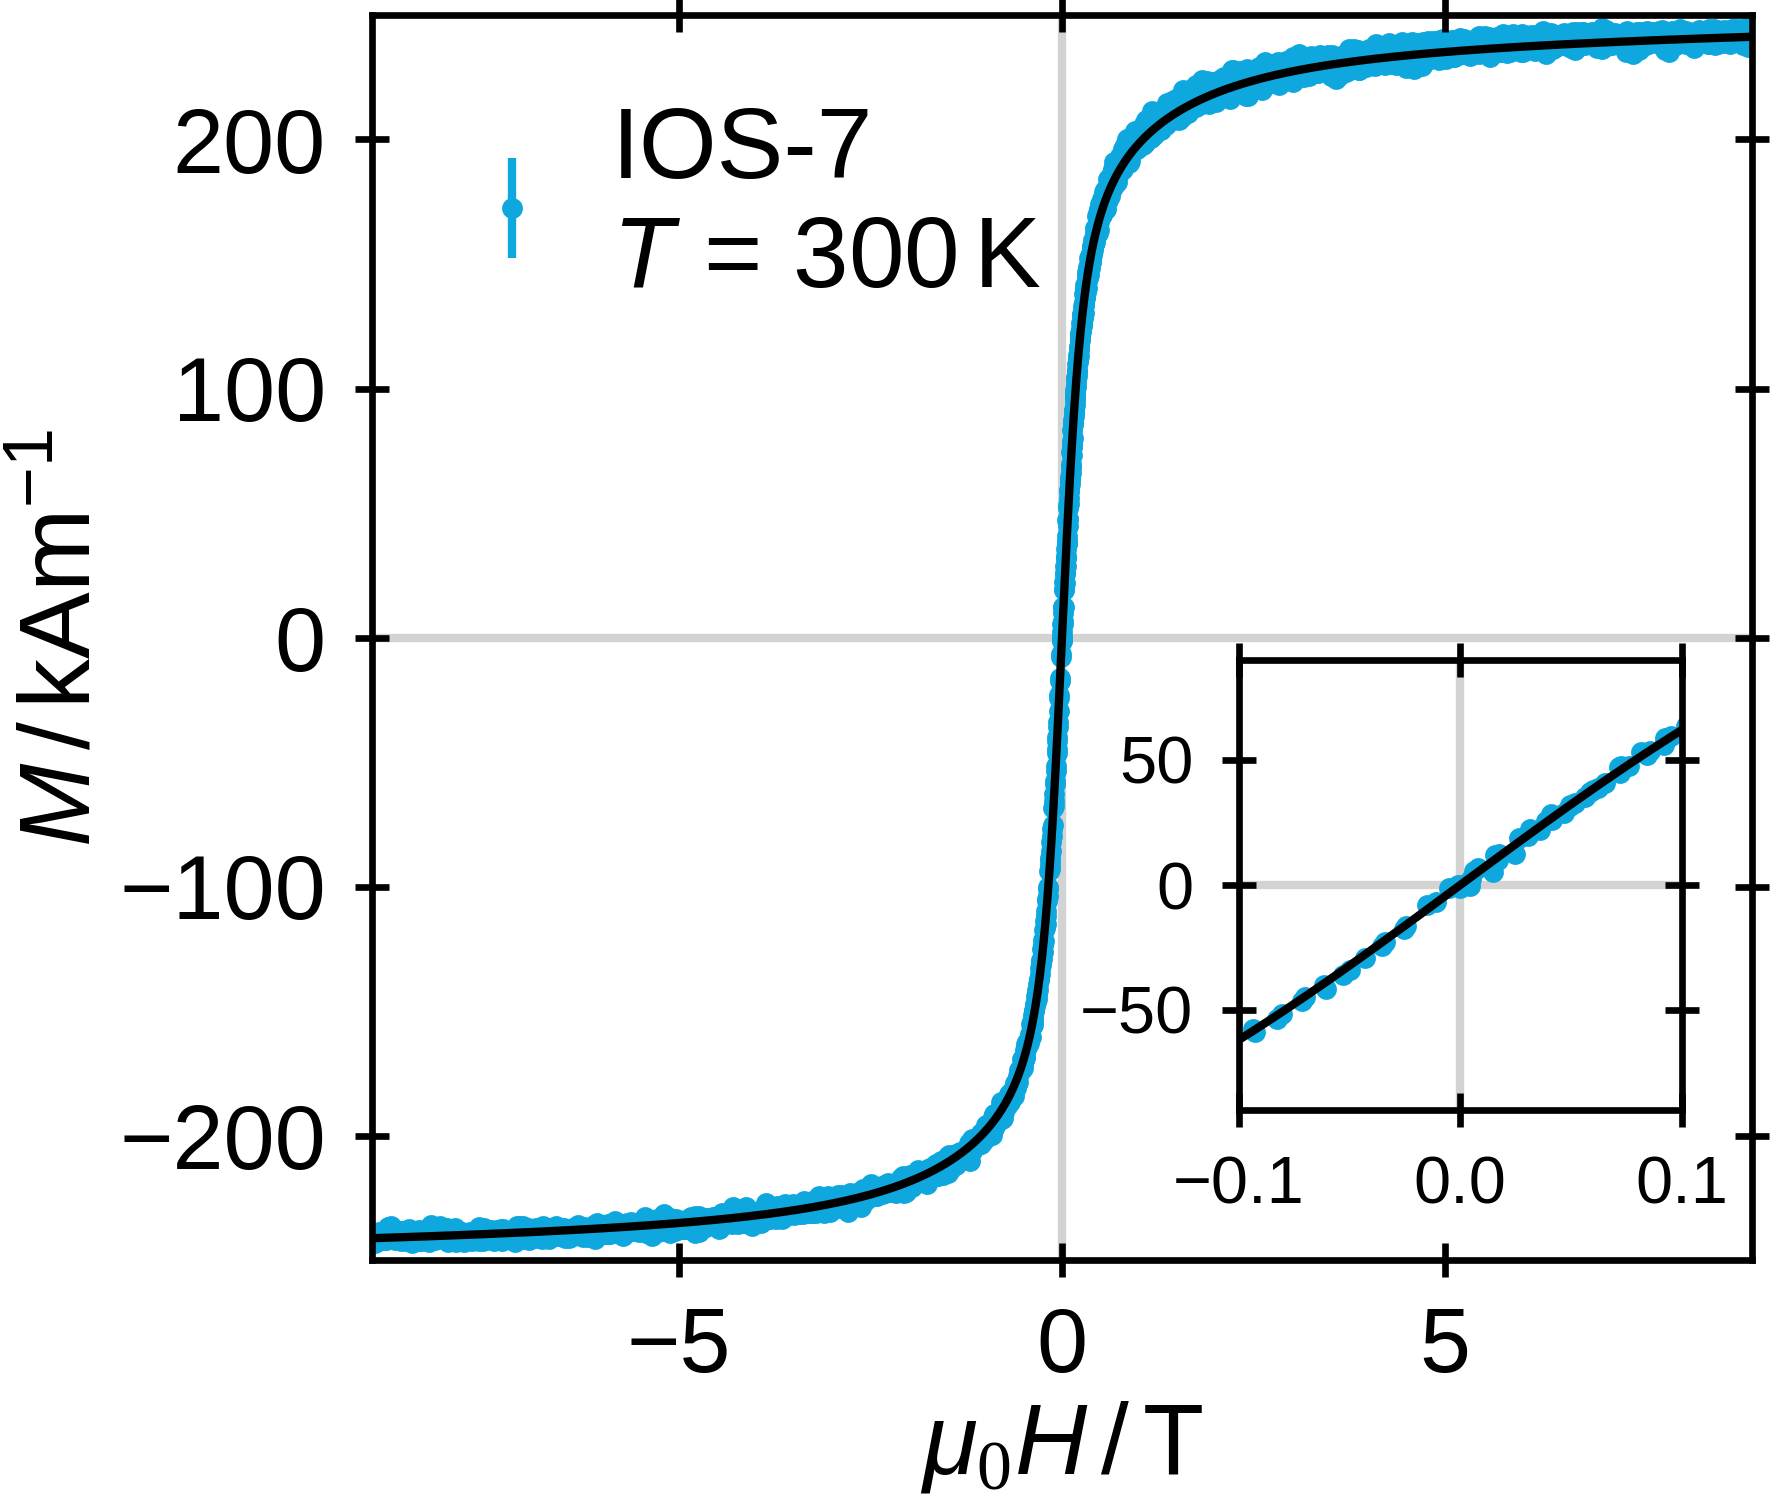
\includegraphics{looselyPackedNP_VSM_IOS-7}
  \caption{\label{fig:looselyPackedNP:nanoparticle:vsm}Room temperature vibrating sample magnetometry for IOS-11 (left) and IOS-7 (right).}
\end{figure}


\begin{table}[tb]
  \centering
  \caption{\label{tab:looselyPackedNP:nanoparticle:vsmSanspol}Parameters for the magnetic structure of the nanospheres obtained from VSM and SANSPOL.}
  \begin{tabular}{ c | l | l }
      & IOS-11 & IOS-7 \\
    \hline
    \multicolumn{3}{c}{VSM}\\
    \hline
    $M_s$
      & $153.0(2) \unit{kAm^{-1}}$
      & $168.0(1) \unit{kAm^{-1}}$\\
    $\mu$
      & $12750(30) \, \mu_B$
      & $3770(40) \, \mu_B$\\
    $\chi$
      & $11.8(2) \mu_0$
      & $10.2(9) \mu_0$\\
    \hline
    $r_m$
      & $5.69(2) \unit{nm}$
      & $3.68(4) \unit{nm}$\\
    \hline
    \multicolumn{3}{c}{SANSPOL}\\
    \hline
    $\rho_\mathrm{mag}$
      & $0.52(3) \unit{10^{-6} \angstrom^{-2}}$
      & $0.33(2) \unit{10^{-6} \angstrom^{-2}}$\\
    $d_\mathrm{dead}$
      & $0.3(1) \unit{nm}$
      & $0 \unit{nm}$\\
    \hline
    $M$
      & $179(10) \unit{kAm^{-1}}$
      & $112(9) \unit{kAm^{-1}}$\\
    \hline
  \end{tabular}
\end{table}

While being in the same order of magnitude, the determined saturation magnetizations from SANSPOL and VSM are not consistent within the error bars for both samples.
This can mostly be attributed to the uncertainty introduced into the VSM data when scaling it to the magnetic volume content.
By estimating the magnetic volume from the magnetic moment and saturation magnetization by
\begin{align}
  V_p^\mathrm{mag} \eq \frac{\mu}{M_s},
\end{align}
a magnetic radius is obtained by
\begin{align}
  r_m \eq \sqrt[3]{\frac{3 V_p}{4 \pi}}.
\end{align}
This is in both cases bigger than the physical particle size, which suggests an under-estimation of the saturation magnetization in VSM.
On the other hand the splitting of the the two polarization channels is very weak for IOS-7, and therefore estimating the parameter for the magnetic scattering length density is limited by the statistical noise.
These limitations have to be kept in mind when comparing the nanoparticle properties in the later step with the properties of a loosely-packed collection of nanoparticles.

\section{Preparation of Loosely-Packed Layers}

\section{Nuclear Structure}

\section{Magnetic Structure}

\section{Emergent Effects}

\section{Model}

\end{document}